% !TeX program = pdflatex
% La escalera de los signos -- el teorema de conteo de raices de Sturm en Lean 4 (version ES).
% Build: pdflatex sturm-lean-es.tex (dos veces, para refs)
% Verificado contra la fuente Lean 2026-06-15 (lake env lean Sturm.lean, exit 0;
% #print axioms Sturm.sturm -> propext, Classical.choice, Quot.sound).
% Toolchain v4.30.0-rc2, Mathlib pin 701fb6e9.

\documentclass[11pt]{article}
\usepackage[T1]{fontenc}
\usepackage[spanish]{babel}
\usepackage{lmodern}
\usepackage{amsmath,amssymb,amsthm,booktabs,graphicx,hyperref}
\usepackage{xurl}
\usepackage[table]{xcolor}
\definecolor{ggteal}{HTML}{1B6F8C}
\definecolor{ggband}{HTML}{DCE7EB}
\definecolor{ggamber}{HTML}{E08A1E}
\usepackage[margin=1in]{geometry}
\usepackage{microtype}
\usepackage{float}
\usepackage[section]{placeins}
\usepackage[most]{tcolorbox}
\usepackage{tikz}
\usetikzlibrary{arrows.meta,positioning}
\graphicspath{{figures/}}
\setlength{\emergencystretch}{4em}
\newtheorem{theorem}{Teorema}
\newtheorem{lemma}{Lema}
\newtheorem{proposition}{Proposici\'on}
\newtheorem{remark}{Observaci\'on}
\newcommand{\lean}[1]{\texttt{#1}}
\newcommand{\R}{\mathbb{R}}
\newcommand{\V}{\mathrm{V}}
\hypersetup{colorlinks=true,linkcolor=ggteal,citecolor=ggteal,urlcolor=ggteal}
\newtcbox{\keybox}{on line,boxrule=0.9pt,colframe=ggteal,colback=ggband!40,
  arc=3pt,left=8pt,right=8pt,top=5pt,bottom=5pt}
\newcommand{\keyeq}[1]{\begin{center}\keybox{$\displaystyle #1$}\end{center}}
\newtcolorbox{recipebox}[1]{colframe=ggamber,colback=ggamber!8,arc=3pt,boxrule=0.8pt,
  title=\textbf{#1},coltitle=white,colbacktitle=ggamber}

\title{\bf La escalera de los signos\\[4pt]
  \large\normalfont El teorema de conteo de ra\'ices de Sturm, verificado por m\'aquina en Lean~4}
\author{Carles Mar\'in\thanks{Formalizado con la asistencia de un sistema de IA (Claude,
Anthropic); la matem\'atica es de Sturm, y toda afirmaci\'on, alcance y limitaci\'on son
responsabilidad del autor. La frontera de la contribuci\'on se expone con claridad en la
Secci\'on~\ref{sec:boundary}, y es el n\'ucleo (\emph{kernel}) de Lean---no la asistente---quien
certifica las pruebas.}\\[3pt]
  \normalsize Investigador independiente\\
  \normalsize \texttt{karlesmarin@gmail.com}}
\date{Junio 2026}

\begin{document}
\maketitle

\begin{abstract}
Presento una formalizaci\'on completa, libre de \lean{sorry}, en Lean~4 sobre Mathlib, del
\emph{teorema de Sturm} (1829): para un polinomio real libre de cuadrados (\emph{squarefree})
$p$ y un intervalo $(a,b]$ cuyos extremos no son ra\'ices, el n\'umero de ra\'ices reales
distintas de $p$ en $(a,b]$ es igual a
\[
  \V(a)-\V(b),
\]
donde $\V(x)$ es el n\'umero de cambios de signo en la \emph{sucesi\'on de Sturm}
$p,\,p',\,-(p \bmod p'),\,\dots$ evaluada en $x$ (descartando los ceros). No se localiza ninguna
ra\'iz; se restan dos enteros. La matem\'atica es enteramente cl\'asica y el resultado ya se hab\'ia
formalizado en otros sistemas (Coq, Isabelle/HOL, HOL~Light); hasta donde s\'e---a partir de
b\'usquedas en Loogle y Mathlib en junio~2026 (Secci\'on~\ref{sec:boundary})---esta es la primera
prueba del teorema de Sturm en Lean. La contribuci\'on es, por tanto, la formalizaci\'on misma y la
maquinaria reutilizable que requiri\'o: una peque\~na teor\'ia de variaci\'on de signo, una
relaci\'on inductiva de ``reducci\'on por flancos'' que desacopla la combinatoria de la cadena de su
\'algebra, y el paso de lo local a lo global, de un \'unico cruce de ra\'iz al conteo en el
intervalo. El teorema central \lean{Sturm.sturm} depende solo de los tres axiomas est\'andar
\lean{propext}, \lean{Classical.choice}, \lean{Quot.sound}. Un subproducto: el conteo de variaciones
de signo de los coeficientes que Mathlib ya ten\'ia (la regla de Descartes) y el que se usa aqu\'i
son, tras desplegar las definiciones, \emph{la misma funci\'on}---de modo que el instrumental se
transfiere literalmente a Descartes.
\end{abstract}

\medskip
\noindent\emph{Qu\'e encontrar\'a aqu\'i.} Es un recorrido breve y guiado, no un manual de
referencia. Se organiza en torno a cuatro preguntas, cada una abre una secci\'on y entrega al lector
la siguiente. La primera pregunta c\'omo es posible que dos enteros cuenten ra\'ices
(Secci\'on~\ref{sec:q1}); la segunda, por qu\'e el conteo solo se mueve en las ra\'ices, y por
exactamente uno (Secci\'on~\ref{sec:q2}); la tercera, d\'onde se resiste de verdad la prueba a
volverse formal, y qu\'e ense\~na esa resistencia (Secci\'on~\ref{sec:q3}); la cuarta, qu\'e queda
gratis una vez el teorema est\'a en la biblioteca (Secci\'on~\ref{sec:q4}). Los lemas que sostienen
todo est\'an reunidos en una tabla (Secci\'on~\ref{sec:blocks}, Tabla~\ref{tab:inventory}); los
l\'imites honestos---la hip\'otesis squarefree, el cuerpo base, lo que \emph{no} se prob\'o, y las
formalizaciones previas en otros sistemas---se exponen sin barniz en la Secci\'on~\ref{sec:boundary};
y la secci\'on de cierre pregunta, a modo de reflexi\'on, qu\'e le falta todav\'ia a este art\'iculo.
Si solo lee dos cosas, lea el Teorema~\ref{thm:sturm} y la Figura~\ref{fig:staircase}; lo dem\'as es
el argumento que los conecta.

\begin{figure}[h]
\centering
\begin{tikzpicture}[
  obj/.style={draw=ggteal,thick,rounded corners=2pt,fill=ggband!40,align=center,
    font=\small,inner sep=5pt,minimum height=10mm},
  q/.style={font=\scriptsize\itshape,text=ggamber!80!black,align=center},
  arr/.style={-{Stealth[length=2.4mm]},thick,ggteal}]
  \node[obj] (seq) {una sucesi\'on\\de restos};
  \node[obj,right=20mm of seq] (count) {un conteo de\\cambios de signo};
  \node[obj,right=20mm of count] (quantum) {una ra\'iz,\\un escal\'on};
  \node[obj,below=14mm of quantum] (glue) {pegar los\\escalones en $(a,b]$};
  \node[obj,left=20mm of glue] (free) {Descartes,\\gratis};
  \node[obj,left=20mm of free,fill=ggamber!25,draw=ggamber] (done)
    {\textbf{Sturm,}\\\textbf{verificado}};
  \draw[arr] (seq) -- node[q,above=1mm] {Q1: \textquestiondown c\'omo\\cuenta una resta?} (count);
  \draw[arr] (count) -- node[q,above=1mm] {Q2: \textquestiondown por qu\'e solo\\en las ra\'ices?} (quantum);
  \draw[arr] (quantum) -- node[q,right=1mm] {Q3: \textquestiondown d\'onde\\se resiste?} (glue);
  \draw[arr] (glue) -- node[q,above=1mm] {Q4: \textquestiondown qu\'e queda\\gratis?} (free);
  \draw[arr] (free) -- (done);
\end{tikzpicture}
\caption{El mapa del lector. De una sucesi\'on de restos a un conteo certificado de ra\'ices y a lo
que produce despu\'es; cada flecha es la pregunta que responde su secci\'on. Cada nodo es un bloque
de Lean libre de \lean{sorry}.}
\label{fig:readermap}
\end{figure}

\section{La pregunta que lo inicia}\label{sec:intro}

\textquestiondown Cu\'antas ra\'ices reales tiene un polinomio entre aqu\'i y all\'a---y puede
decirse sin encontrar ni una sola de ellas?

La pregunta es antigua y fue, durante mucho tiempo, genuinamente dif\'icil. La regla de los signos de
Descartes (1637)~\cite{descartes} lee una \emph{cota} a partir de los signos de los coeficientes;
Budan y Fourier (principios del siglo~XIX)~\cite{bf} la afinaron a una cota para un intervalo; pero
una cota no es un conteo, y la distancia entre ambos resisti\'o a los mejores analistas de la \'epoca.
La cerr\'o en 1829 un joven Charles-Fran\c{c}ois Sturm, que anunci\'o---y en 1835 public\'o
\'integramente~\cite{sturm}---un procedimiento que devuelve el n\'umero \emph{exacto} de ra\'ices
reales distintas en cualquier intervalo, sin aproximaci\'on alguna y sin localizar ra\'ices. El
m\'etodo fue celebrado de inmediato; es el antepasado del aislamiento de ra\'ices reales, de la
descomposici\'on cil\'indrica algebraica y de los procedimientos de decisi\'on para la teor\'ia de
primer orden de los reales que crecieron a partir del trabajo de Tarski. El problema de
contar ra\'ices reales de forma exacta qued\'o, en efecto, resuelto por una resta.

El mecanismo es un peque\~no giro sobre algo a\'un m\'as antiguo. El algoritmo de Euclides, aplicado a
$p$ y su derivada $p'$, produce una sucesi\'on de restos; el giro de Sturm es negar cada resto al
formarlo,
\[
  p_0=p,\quad p_1=p',\quad p_{k+1}=-(p_{k-1}\bmod p_k),
\]
deteni\'endose cuando el resto se anula. Ll\'amese a esto la \emph{sucesi\'on de Sturm}. Para un
punto $x$ que no es ra\'iz de ning\'un miembro, sea $\V(x)$ el n\'umero de veces que cambia el signo
al leer $p_0(x),p_1(x),\dots$ de izquierda a derecha, ignorando los ceros. El teorema de Sturm afirma
que $\V$ es, disfrazado, un contador de ra\'ices:
\keyeq{\#\{\text{ra\'ices reales distintas de }p\text{ en }(a,b]\}\;=\;\V(a)-\V(b).}

El resultado es de manual, y se ha verificado por m\'aquina antes: en Coq, como parte de la
construcci\'on de los n\'umeros algebraicos reales de Cohen~\cite{cohen}; en Isabelle/HOL, por
Eberl~\cite{eberl} y---en la forma m\'as fina de Sturm--Tarski, v\'ia el \'indice de
Cauchy---por Li y Paulson~\cite{litarski,libudan}; y en HOL~Light. Lo que no se hab\'ia hecho, hasta
ahora, es en \emph{Lean}. Mathlib, la biblioteca sobre la que se construye buena parte de la
matem\'atica formalizada contempor\'anea, lleva la regla de los signos de Descartes (la funci\'on
\lean{Polynomial.signVariations}) pero no la sucesi\'on de Sturm ni el teorema de Sturm. Este
art\'iculo cubre esa carencia. Quiero ser exacto: es un primero-en-Lean y no un primero-en-cualquier
sistema;\footnote{Reivindicaci\'on de prioridad basada en b\'usquedas en Loogle y un \lean{grep} de
Mathlib a junio~2026; las formalizaciones previas en Coq, Isabelle/HOL y HOL~Light se acreditan en la
Secci\'on~\ref{sec:boundary}.} el valor est\'a en a\~nadir una herramienta fundamental a una
biblioteca que no la ten\'ia, y en las piezas reutilizables que la prueba deja tras de s\'i.

No llegu\'e a ello propon\'endome demostrar el teorema de Sturm, sino preguntando, una y otra vez,
qu\'e resultados cl\'asicos le faltan a\'un a una biblioteca madura---y el de Sturm, situado de lleno
en el conteo de ra\'ices reales, estaba entre las ausencias m\'as llamativas. El resto del art\'iculo
es el camino desde la ausencia hasta el teorema, contado como las cuatro preguntas que un lector
cuidadoso probablemente se haga, una tras otra.

\section{Q1: \textquestiondown c\'omo puede una resta de enteros contar ra\'ices?}\label{sec:q1}

\emph{Apunte hist\'orico.} La sucesi\'on y el enunciado del conteo son del propio
Sturm~(\cite{sturm}; el tratamiento moderno es el de Basu--Pollack--Roy~\cite{bpr}). Nada en esta
secci\'on es matem\'atica nueva; el Lean est\'a en \lean{Sturm.lean}, definiciones \lean{sturmSeq} y
\lean{signVarAt}.

Precisemos los dos ingredientes. La sucesi\'on de Sturm se construye con la recursi\'on euclidiana
negada de arriba; en Lean es \lean{sturmSeq p}, una \lean{List} de polinomios producida por una
auxiliar \lean{sturmAux} que recurre sobre el grado del divisor y termina porque cada resto tiene
grado estrictamente menor. El conteo de signos es
\[
  \V(x)\;=\;\lean{signVarAt (sturmSeq p) x},
\]
definido como el n\'umero de cambios de signo en la lista de signos evaluados
$\big(\mathrm{sign}\,p_0(x),\mathrm{sign}\,p_1(x),\dots\big)$ tras borrar los ceros. (En la fuente
Lean ese borrar-y-contar se expresa con \lean{List.destutter}; una forma recursiva equivalente y m\'as
c\'omoda, \lean{signChanges}, se prueba igual a aquella y es la que usa el resto del desarrollo.)

\begin{theorem}[teorema de Sturm, en Lean~4; \lean{Sturm.sturm}]\label{thm:sturm}
Sea $p$ un polinomio real squarefree y $a<b$ con $p(a)\ne0$ y $p(b)\ne0$. Entonces
\keyeq{\V(a)-\V(b)\;=\;\#\{x : a<x\le b,\ p(x)=0\},}
el n\'umero de ra\'ices reales \emph{distintas} de $p$ en el intervalo semiabierto $(a,b]$. El
enunciado es libre de \lean{sorry}; \lean{\#print axioms Sturm.sturm} reporta solo \lean{propext},
\lean{Classical.choice}, \lean{Quot.sound}.
\end{theorem}

Que una diferencia de dos enteros sea igual a un conteo es, a primera vista, un peque\~no milagro, as\'i
que conviene verlo ocurrir una vez a mano.

\emph{Un caso comprobable a mano.} Tomemos $p(x)=x^3-x=x(x-1)(x+1)$, con ra\'ices $-1,0,1$. La
recursi\'on euclidiana negada da la sucesi\'on de cuatro t\'erminos
\[
  p_0=x^3-x,\quad p_1=3x^2-1,\quad p_2=\tfrac{2}{3}x,\quad p_3=1.
\]
Le\'amos los signos en los dos extremos de $(-2,2]$:
\[
  \begin{array}{c|cccc|c}
   x & p_0 & p_1 & p_2 & p_3 & \V \\\hline
   -2 & - & + & - & + & 3 \\
   \phantom{-}2 & + & + & + & + & 0
  \end{array}
\]
de modo que $\V(-2)-\V(2)=3-0=3$, exactamente el n\'umero de ra\'ices en $(-2,2]$. N\'otese que no se
calcul\'o ninguna ra\'iz; solo se leyeron signos. (Cada entrada de esta tabla se recomprueba en
aritm\'etica exacta con el guion que acompa\~na a la Figura~\ref{fig:staircase}.)

La imagen tras la tabla es la que da nombre a este art\'iculo. Dib\'ujese $\V(x)$ a medida que $x$
barre la recta: es una \emph{escalera}, plana casi en todas partes y que baja en uno cuando $x$ pasa
por cada ra\'iz de $p$ (Figura~\ref{fig:staircase}; la Tabla~\ref{tab:signs} la lee punto a punto). El
teorema de Sturm no es entonces sino leer el descenso total de la escalera entre $a$ y $b$. Toda la
dificultad---y todo el contenido de las dos secciones siguientes---est\'a en probar que la escalera
tiene exactamente esta forma: que es plana salvo en las ra\'ices, y que cada escal\'on mide
exactamente uno.

\begin{figure}[t]
\centering
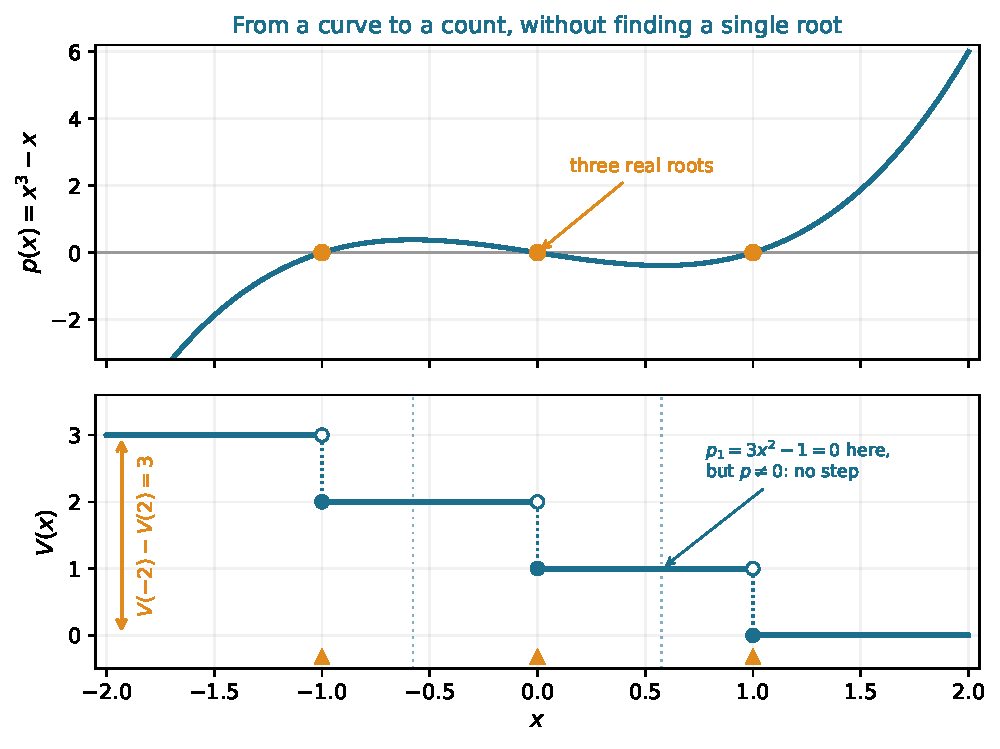
\includegraphics[width=0.93\textwidth]{sturm_fig1_staircase}
\caption{La escalera de los signos para $p=x^3-x$. \emph{Arriba:} el polinomio y sus tres ra\'ices
reales. \emph{Abajo:} el conteo $\V(x)$ es plano salvo en las ra\'ices $-1,0,1$, donde baja en
exactamente uno (c\'irculo abierto = el valor justo a la izquierda, c\'irculo lleno = el valor en la
ra\'iz, en el escal\'on inferior). En un cero de un miembro \emph{interior} de la sucesi\'on---aqu\'i
$p_1=3x^2-1$ se anula en $x=\pm1/\sqrt3$ (gu\'ias punteadas), puntos donde $p$ no es cero---la
escalera \emph{no} se mueve. El descenso total sobre $(-2,2]$ (la flecha \'ambar) es el n\'umero de
ra\'ices all\'i. El guion generador comprueba cada signo y conteo dibujado contra aritm\'etica
racional exacta antes de dibujar. \emph{(Las etiquetas de la figura est\'an en ingl\'es, compartidas
con la edici\'on inglesa.)}}
\label{fig:staircase}
\end{figure}

\begin{table}[t]
\centering\small
\rowcolors{2}{ggband!35}{white}
\begin{tabular}{@{}rccccr@{}}
\toprule
\rowcolor{ggteal!18} $x$ & $p_0=x^3{-}x$ & $p_1=3x^2{-}1$ & $p_2=\tfrac23 x$ & $p_3=1$ & $\V(x)$ \\
\midrule
$-2$            & $-$ & $+$ & $-$ & $+$ & $3$ \\
$-1$ {\scriptsize(ra\'iz)} & $0$ & $+$ & $-$ & $+$ & $2$ \\
$-\tfrac12$     & $+$ & $-$ & $-$ & $+$ & $2$ \\
$-\tfrac{1}{\sqrt3}$ {\scriptsize($p_1{=}0$)} & $+$ & $0$ & $-$ & $+$ & $2$ \\
$0$ {\scriptsize(ra\'iz)}  & $0$ & $-$ & $0$ & $+$ & $1$ \\
$\tfrac{1}{\sqrt3}$ {\scriptsize($p_1{=}0$)}  & $-$ & $0$ & $+$ & $+$ & $1$ \\
$1$ {\scriptsize(ra\'iz)}  & $0$ & $+$ & $+$ & $+$ & $0$ \\
$2$             & $+$ & $+$ & $+$ & $+$ & $0$ \\
\bottomrule
\end{tabular}
\caption{El mismo ejemplo le\'ido en los signos. Cada fila eval\'ua los cuatro miembros de la cadena
y cuenta los cambios de signo (ceros omitidos). $\V$ baja en uno en cada \emph{ra\'iz} de $p$ y no
cambia al cruzar cada cero del miembro \emph{interior} $p_1$ (las filas $\tfrac{1}{\sqrt3}$)---los
dos comportamientos que explica la Secci\'on~\ref{sec:q2}. Toda la tabla se regenera y comprueba en
aritm\'etica exacta con el guion de la figura.}
\label{tab:signs}
\end{table}

\section{Q2: \textquestiondown por qu\'e el conteo solo se mueve en las ra\'ices, y por exactamente
uno?}\label{sec:q2}

\emph{Apunte hist\'orico.} El an\'alisis local---qu\'e le pasa a $\V$ cuando $x$ cruza un punto---es
el coraz\'on de toda prueba del teorema de Sturm desde la de Sturm. Los dos hechos en que se apoya (un
miembro y sus vecinos no pueden anularse juntos; miembros consecutivos son antipodales en un cero del
que est\'a entre ellos) son cl\'asicos; el Lean est\'a en los lemas \lean{not\_common\_root},
\lean{sign\_neighbours\_opposite\_at\_interior\_root} y \lean{signVarAt\_drop\_at\_critical\_point}.

Ll\'amese \emph{cr\'itico} a un punto donde se anula alg\'un miembro de la sucesi\'on. Lejos de los
puntos cr\'iticos cada miembro conserva su signo (un polinomio no puede cambiar de signo sin una
ra\'iz, por el teorema del valor intermedio), as\'i que $\V$ es localmente constante: este es
\lean{signVarAt\_eq\_of\_no\_root}, y es por lo que la escalera es plana entre cr\'iticos. Toda la
acci\'on est\'a en los puntos cr\'iticos, y los hay de dos clases.

\emph{Las ra\'ices de $p$.} Sup\'ongase $p(c)=0$. Como $p$ es squarefree no comparte ra\'iz con $p'$,
luego $p'(c)\ne0$, y justo a izquierda y derecha de $c$ el polinomio $p$ toma signos opuestos (cruza
el cero transversalmente, con el signo de $p'(c)$ a la derecha y el opuesto a la izquierda). El primer
par de la sucesi\'on, $(p,p')$, cambia por tanto en exactamente uno su n\'umero de acuerdos internos
de signo al cruzar $c$. Este es el \'unico escal\'on de la escalera, aislado en Lean como la ca\'ida
del par de cabeza \lean{signVarAt\_cons\_head\_drop}, alimentado por los lemas de transversalidad
\lean{sign\_eval\_eq\_sign\_deriv\_right} y \lean{sign\_eval\_eq\_neg\_sign\_deriv\_left}.

\emph{Los dem\'as puntos cr\'iticos.} Un miembro $p_k$ con $1\le k$ tambi\'en puede anularse en $c$
sin que $p$ lo haga. Aqu\'i est\'a el mecanismo que hace funcionar el teorema de Sturm, y merece
enunciarse como el lema indispensable:
\begin{lemma}[vecinos antipodales; \lean{sign\_neighbours\_opposite\_at\_interior\_root}]
\label{lem:antipodal}
Si miembros consecutivos $p_{k-1},p_k$ son coprimos y $p_k(c)=0$, entonces $p_{k-1}(c)$ y
$p_{k+1}(c)$ son ambos no nulos y de signo \emph{opuesto}.
\end{lemma}
La raz\'on es una consecuencia de una l\'inea de la recursi\'on definitoria $p_{k+1}=-(p_{k-1}\bmod
p_k)$ evaluada en una ra\'iz de $p_k$: all\'i $p_{k-1}(c)=-p_{k+1}(c)$ (lema
\lean{eval\_eq\_neg\_next\_of\_root}), y ninguno puede ser cero porque polinomios coprimos no comparten
ra\'iz (\lean{not\_common\_root}). En consecuencia, sea cual sea el signo que adopte $p_k$ a cada lado
de $c$---y sea positivo, negativo, o exactamente cero \emph{en} $c$---queda entre dos vecinos fijos y
opuestos, y un valor encajado entre signos opuestos no aporta nada al conteo de cambios de signo, sea
cual sea. El miembro de en medio es invisible. Por eso un cero de un miembro interior no mueve la
escalera en absoluto (las marcas $p_1=0$ de la Figura~\ref{fig:staircase}); la coprimalidad de
miembros consecutivos, que se propaga por la cadena desde $\gcd(p,p')=1$, lo garantiza en todas
partes.

Juntando las dos clases se obtiene el cuanto por punto---la altura de un \'unico escal\'on:
\begin{proposition}[un punto cr\'itico; \lean{signVarAt\_drop\_at\_critical\_point}]
\label{prop:quantum}
Si $c$ es el \'unico punto cr\'itico en $[a,b]$ y $p(a),p(b)\ne0$, entonces
\[
  \V(a)=\V(b)+\begin{cases}1 & p(c)=0,\\ 0 & p(c)\ne0.\end{cases}
\]
\end{proposition}
La prueba es donde la formalizaci\'on se gana el sueldo, y es el tema de la secci\'on siguiente,
porque hacerla rigurosa exigi\'o un recurso que el manual no necesita.

\section{Q3: \textquestiondown d\'onde se resiste la prueba a volverse formal?}\label{sec:q3}

\emph{Apunte hist\'orico.} Sobre el papel, ``los miembros interiores se cancelan y solo importa $p$''
es una frase. Hecha formal, es el \'unico paso genuinamente estructural, porque la cancelaci\'on ha de
ejecutarse \emph{a lo largo de una lista cuya forma es ella misma recursiva}. El recurso que lo
resuelve (\lean{FlankReduce} y \lean{flankReduce\_chain\_walk}) es, hasta donde s\'e, la \'unica parte
de este desarrollo sin un antecedente directo de manual---no un teorema nuevo, sino una pieza de
ingenier\'ia de pruebas.

La dificultad es precisa. Para comparar $\V(a)$ con $\V(b)$ a trav\'es de un \'unico punto cr\'itico
$c$, uno quiere borrar de la lista de signos, en \emph{ambos} $a$ y $b$, cada miembro interior que se
anula en $c$---cada uno encajado entre vecinos opuestos, de modo que borrarlo no cambia nada
(Lema~\ref{lem:antipodal})---y observar entonces que las dos listas podadas difieren solo en la cabeza
$p$. Pero ``borrar cada tal miembro'' es una inducci\'on sobre la sucesi\'on de Sturm, y las
hip\'otesis que justifican un borrado (los vecinos flanqueantes son no nulos y opuestos \emph{en el
punto de evaluaci\'on}) van entretejidas en la propia estructura de la cadena. La combinatoria de
podar una lista y el \'algebra de por qu\'e cada poda es l\'icita est\'an enredadas, y una prueba
honesta debe separarlas.

La separaci\'on es una relaci\'on inductiva. Dir\'e que una lista de signos \emph{se reduce por
flancos} a otra cuando la segunda se obtiene de la primera borrando repetidamente una entrada situada
entre dos signos no nulos opuestos:
\begin{recipebox}{El desacoplo (receta)}
\lean{FlankReduce}~$L\;L'$ se cumple cuando $L'$ se obtiene de $L$ borrando entradas atrapadas cada
una entre dos signos no nulos opuestos: un paso lleva
$\textit{pre}\mathbin{+\!\!+}[a,m,b]\mathbin{+\!\!+}\textit{rest}$ a
$\textit{pre}\mathbin{+\!\!+}[a,b]\mathbin{+\!\!+}\textit{rest}$ siempre que $a,b\ne0$ y $a\ne b$, y
la relaci\'on es el cierre reflexivo de iterarlo. Dos hechos reparten entonces el trabajo con
limpieza. \emph{Combinatorio:} la reducci\'on por flancos
preserva el n\'umero de cambios de signo (\lean{FlankReduce.signChanges\_eq})---esto es pura
\'algebra de listas, sin polinomios. \emph{Estructural:} la lista de signos evaluados de la cadena de
Sturm en cualquier punto se reduce por flancos a la cadena sin sus anuladores interiores en $c$
(\lean{flankReduce\_chain\_walk})---esta es la inducci\'on sobre la cadena, que suministra las
hip\'otesis de flanco desde la coprimalidad y la constancia local del signo, y nada m\'as.
\end{recipebox}

\begin{figure}[t]
\centering
\begin{tikzpicture}[
  s/.style={draw=ggteal,rounded corners=1.5pt,minimum size=7mm,inner sep=2pt,font=\small,fill=white},
  sm/.style={draw=ggamber,rounded corners=1.5pt,minimum size=7mm,inner sep=2pt,font=\small,
    fill=ggamber!12,text=ggamber!80!black},
  arr/.style={-{Stealth[length=2.2mm]},thick,ggteal},
  lbl/.style={font=\scriptsize\itshape,text=ggteal!75!black}]
  \node[font=\bfseries\small,text=ggteal] at (-0.1,1.15) {(a) el \'atomo};
  \node[s] (a1) at (0,0) {$+$};
  \node[sm] (am) at (0.75,0) {$?$};
  \node[s] (a2) at (1.5,0) {$-$};
  \node[s] (b1) at (3.4,0) {$+$};
  \node[s] (b2) at (4.15,0) {$-$};
  \draw[arr] (2.0,0) -- (2.95,0);
  \node[lbl,align=center] at (2.48,0.5) {borrar};
  \node[font=\scriptsize,align=center,text width=5.2cm] at (2.1,-0.95)
    {un medio entre dos signos \emph{opuestos} es invisible al conteo---sea $+$, $-$ o $0$};
  \node[font=\bfseries\small,text=ggteal] at (8.6,1.55) {(b) los dos extremos coinciden};
  \node[lbl] at (6.05,0.95) {en $a$:};
  \node[s,fill=ggband!50] (pa) at (6.7,0.95) {$\mathrm{sg}\,p(a)$};
  \node[s] at (7.95,0.95) {$+$};
  \node[sm] at (8.55,0.95) {$\ast$};
  \node[s] at (9.15,0.95) {$-$};
  \node[s] at (9.75,0.95) {$\cdots$};
  \node[lbl] at (6.05,0.05) {en $b$:};
  \node[s,fill=ggband!50] (pb) at (6.7,0.05) {$\mathrm{sg}\,p(b)$};
  \node[s] at (7.95,0.05) {$+$};
  \node[sm] at (8.55,0.05) {$\ast$};
  \node[s] at (9.15,0.05) {$-$};
  \node[s] at (9.75,0.05) {$\cdots$};
  \node[s,fill=ggamber!18,draw=ggamber] (red) at (8.4,-1.0) {$p\,\mathbin{:\!:}$ no-anuladores};
  \draw[arr] (8.6,0.55) -- (8.5,-0.7);
  \draw[arr] (8.6,-0.35) -- (8.5,-0.78);
  \node[font=\scriptsize,align=center,text width=5.6cm] at (8.4,-1.75)
    {misma cadena podada en ambos extremos; solo la cabeza $\mathrm{sg}\,p$ puede diferir, y lo hace
     \emph{si y solo si} $p(c)=0$};
\end{tikzpicture}
\caption{El desacoplo de la Secci\'on~\ref{sec:q3}. \emph{(a)} El \'atomo combinatorio: una entrada
flanqueada por signos no nulos opuestos ($\ast$, el anulador interior) puede borrarse sin cambiar el
n\'umero de cambios de signo, sea cual sea su propio valor. \emph{(b)} Aplicado a lo largo de la
cadena en ambos extremos, todo anulador interior en $c$ se borra, de modo que las listas de signos en
$a$ y en $b$ se reducen a la \emph{misma} cadena podada; la \'unica entrada que puede diferir es la
cabeza $\mathrm{sg}\,p$. El \'algebra de la cadena suministra las hip\'otesis de ``vecinos
opuestos''; el conteo lo mueve \lean{FlankReduce}, que nunca menciona un polinomio.}
\label{fig:flank}
\end{figure}

Separadas las dos mitades, la Proposici\'on~\ref{prop:quantum} se vuelve ensamblaje: la lista de
signos de la cadena se reduce por flancos, en $a$ y en $b$ por igual, a la \emph{misma} cadena podada
$p\mathbin{:\!:}(\text{no-anuladores})$; en esa cadena podada solo $p$ puede cambiar de signo entre
$a$ y $b$, de modo que el cambio en $\V$ es la \'unica ca\'ida de cabeza cuando $p(c)=0$ y nada en
otro caso. La estructura de la cadena entra solo para entregar al lema combinatorio sus hip\'otesis;
el conteo lo mueve una relaci\'on que nada sabe de polinomios.

\emph{Lo que la m\'aquina me hizo enunciar bien.} Hay aqu\'i una lecci\'on m\'as callada, del tipo
que un asistente de pruebas extrae bien. La prueba cl\'asica supone t\'acitamente ``posici\'on
gen\'erica'': que ning\'un miembro de la sucesi\'on se anula en los extremos $a,b$, y que siempre se
puede deslizar a tales puntos. Formalizar proh\'ibe el gesto a mano---y resulta que la reducci\'on por
flancos ya trata los casos inc\'omodos gratis. Un miembro que se anula justo en un punto de
evaluaci\'on sigue encajado all\'i entre vecinos opuestos, as\'i que sigue borr\'andose por la misma
relaci\'on; la cadena podada es la misma; el conteo no se ve afectado. Por eso prob\'e el lema por
punto (Proposici\'on~\ref{prop:quantum}) para un punto cr\'itico en cualquier lugar del intervalo
cerrado $[a,b]$, extremos incluidos, y no solo estrictamente dentro---y los casos degenerados que el
manual pasa por alto se despachan con la misma l\'inea que el caso principal. El principio
transferible es el mismo que extrajo el art\'iculo compa\~nero sobre las desigualdades de
Newton~\cite{newton}: enunciar un paso al nivel m\'as d\'ebil que sea honesto a menudo disuelve, en
vez de multiplicar, los casos l\'imite.

\emph{De un escal\'on a toda la escalera.} El enunciado global es entonces una inducci\'on sobre el
n\'umero de puntos cr\'iticos en $(a,b]$ (\lean{Sturm.sturm}; los cr\'iticos son las ra\'ices del
producto de todos los miembros, un polinomio no nulo, luego finito). Qu\'itese el mayor punto cr\'itico
$c$; el\'ijase un separador no cr\'itico $d$ justo por debajo de \'el---existe porque los cr\'iticos
son finitos y los reales son densos; apl\'iquese el cuanto por punto en $[d,b]$, donde $c$ es el
\'unico punto cr\'itico; y rec\'urrase en $[a,d]$, que tiene uno menos. El intervalo semiabierto
$(a,b]$ se parte como $(a,d]\sqcup(d,b]$, el conteo de ra\'ices se suma, y la contribuci\'on por
punto---uno cuando $p(c)=0$, cero en otro caso---coincide con el n\'umero de ra\'ices de $p$ en el
trozo retirado. El conteo global se ensambla a partir de los escalones por punto.

\begin{remark}[el patr\'on tras \lean{FlankReduce}]\label{rem:pattern}
Conviene abstraer \lean{FlankReduce} de su uso aqu\'i. Es una instancia de un esquema recurrente: un
invariante num\'erico---el conteo de cambios de signo---preservado bajo borrados autorizados por una
condici\'on lateral puramente \emph{local} (una entrada entre dos signos no nulos opuestos). Podr\'ia
llamarse un \emph{invariante de conteo bajo poda admisible}. Su valor es justamente el desacoplo
mostrado arriba: la combinatoria global se reduce a (i)~un lema de preservaci\'on de un paso, sin
polinomios y probado una vez (\lean{FlankReduce.signChanges\_eq}), y (ii)~un recorrido estructural que
certifica la condici\'on lateral de cada borrado desde el problema concreto
(\lean{flankReduce\_chain\_walk}). La misma separaci\'on deber\'ia aplicarse dondequiera que un
recuento sea invariante bajo borrados localmente justificados---la sucesi\'on de derivadas de
Budan--Fourier, o en general cualquier sistema de reescritura con un conteo conservado. Pruebo solo la
instancia que Sturm necesit\'o y no desarrollo la teor\'ia general; pero la forma es general, y
nombrarla---en vez de incrustar los borrados en la inducci\'on de la cadena---es lo que hizo modular la
prueba. Si ``invariancia de un recuento bajo borrado localmente autorizado'' merece ser una
abstracci\'on de Mathlib por derecho propio es la pregunta abierta que m\'as me interesa llevar
adelante (Secci\'on~\ref{sec:questions}).
\end{remark}

\section{Q4: \textquestiondown qu\'e queda gratis una vez certificado el teorema?}\label{sec:q4}

\emph{Apunte hist\'orico.} El conteo de Sturm de variaciones de signo en un \emph{intervalo} y el
conteo de Descartes de variaciones de signo en los \emph{coeficientes} (1637) suelen ense\~narse como
primos. En Lean resultan ser, tras desplegar, la misma funci\'on---una peque\~na sorpresa que la
formalizaci\'on sac\'o a la luz gratis. El Lean es \lean{signVariations\_eq\_signChanges}.

Mathlib ya ten\'ia la regla de los signos de Descartes, expresada por \lean{Polynomial.signVariations},
el n\'umero de cambios de signo en la lista de coeficientes de un polinomio. El conteo construido
aqu\'i para el teorema de Sturm, \lean{signChanges}, est\'a definido sobre una lista arbitraria de
signos. Al desplegar ambos, coinciden exactamente:
\keyeq{\lean{P.signVariations}\;=\;\lean{signChanges}\,(\lean{P.coeffList.map sign}),}
una prueba que es, literalmente, \lean{rfl}. La consecuencia es pr\'actica: el instrumental reunido
para Sturm---los ceros son invisibles al conteo, una entrada entre vecinos opuestos se cancela, la
recursi\'on por cabeza, la paridad (una lista sin ceros tiene un n\'umero par de cambios de signo si y
solo si sus extremos coinciden)---no es espec\'ifico de Sturm. Se transfiere literalmente a Descartes,
y los dos teoremas cl\'asicos de variaci\'on de signo comparten ahora en la biblioteca un \'unico
n\'ucleo combinatorio en vez de dos paralelos. Una peque\~na unificaci\'on, pero exactamente del tipo
que una biblioteca formal deber\'ia acumular.

Otras dos cosas caen sin trabajo nuevo. Primero, el \emph{aislamiento de ra\'ices}: aplicar el teorema
a $(a,b]$ y a sus dos mitades repetidamente a\'isla cada ra\'iz real en un intervalo tan peque\~no
como se quiera, el uso algor\'itmico por el que el m\'etodo de Sturm es m\'as conocido. Segundo, los
\emph{bloques de construcci\'on} mismos---la constancia local del signo, el lema de vecinos
antipodales, los hechos estructurales sobre la sucesi\'on (miembros consecutivos coprimos, la
recursi\'on que relaciona cada terna, el \'ultimo miembro una constante no nula)---son reutilizables
para cualquier trabajo futuro de conteo de ra\'ices reales en Lean: el teorema de Budan--Fourier, el
conteo de Sturm--Tarski con multiplicidad~\cite{libudan}, o un desarrollo del \'indice de Cauchy
beber\'ian de las mismas piezas.

\section{Qu\'e habilita un conteo de ra\'ices certificado}\label{sec:enables}

La matem\'atica aqu\'i tiene dos siglos; la raz\'on para ponerla en Lean es lo que desbloquea
\emph{dentro} de la biblioteca, donde un conteo exacto y verificado de ra\'ices sencillamente no
exist\'ia. Conviene ser concreto, porque un lema fundamental vale en proporci\'on a lo que se apoya
en \'el. Cuatro cosas se vuelven alcanzables que antes no lo eran, en orden aproximado de distancia
a lo que se prueba.

\emph{Aislamiento de ra\'ices reales.} El uso algor\'itmico cl\'asico del teorema de Sturm es aislar
cada ra\'iz real en un intervalo tan estrecho como se quiera: aplicar el conteo a $(a,b]$, bisecar,
recurrir, y detener una rama cuando su conteo es $0$ (sin ra\'iz) o $1$ (exactamente una). Como el
conteo aqu\'i es \emph{exacto}, no una cota, la recursi\'on termina demostrablemente con una ra\'iz
por intervalo. Todos los ingredientes est\'an ya probados---el conteo, la constancia local, la
finitud del conjunto cr\'itico---as\'i que lo que queda es la envoltura recursiva y su terminaci\'on,
no matem\'atica nueva. Esto convierte el teorema de un enunciado en un \emph{procedimiento}
certificado, la forma en que el m\'etodo de Sturm se usa de verdad.

\emph{El teorema de Budan--Fourier.} Budan y Fourier cuentan variaciones de signo en la sucesi\'on
de \emph{derivadas} $p,p',p'',\dots$ y acotan (con la paridad correcta) las ra\'ices en un
intervalo. Es la misma aritm\'etica de variaci\'on de signo que aqu\'i, sobre otra sucesi\'on; el
instrumental construido para Sturm---ceros invisibles, la recursi\'on por cabeza, y en particular el
lema de paridad \lean{wallCount\_even\_iff\_endpoints}---se transfiere directamente. Mathlib ya
ten\'ia la regla de Descartes (\lean{signVariations}); Budan--Fourier se sit\'ua entre Descartes y
Sturm, y las piezas para alcanzarlo est\'an ahora en su sitio.

\emph{Sturm--Tarski y el \'indice de Cauchy.} El teorema m\'as fino de Sturm--Tarski cuenta ra\'ices
de $p$ \emph{ponderadas} por el signo de un segundo polinomio $q$ sobre ellas---la ``consulta de
Tarski'' $\sum_{p(x)=0}\operatorname{sign} q(x)$---que es igual al \'indice de Cauchy de $p'q/p$ (el
caso b\'asico $q=1$, el \'indice de Cauchy de $p'/p$, es el propio conteo de Sturm). Este es el motor
del conteo de ra\'ices \emph{con multiplicidad}, del caso no squarefree, y en \'ultima instancia de la eliminaci\'on de
cuantificadores de Tarski para los reales. La sucesi\'on de restos con signo y el conteo de
variaci\'on ensamblados aqu\'i son precisamente su sustrato; el desarrollo en Isabelle de
Sturm--Tarski~\cite{litarski,libudan} se construye sobre los mismos dos objetos. Una versi\'on en
Lean extender\'ia, no reiniciar\'ia, el presente fichero.

\emph{Procedimientos de decisi\'on sobre los reales.} El conteo y aislamiento de ra\'ices reales en
una variable son el caso base de la descomposici\'on cil\'indrica algebraica y de los procedimientos
de decisi\'on para la teor\'ia de primer orden de los cuerpos realmente cerrados
(Tarski--Seidenberg). Para Lean en concreto, este es el cimiento que faltaba bajo cualquier futura
respuesta \emph{certificada} a ``\textquestiondown tiene este polinomio una ra\'iz en este rango, y
cu\'antas?''---un certificado comprobable en el que una t\'actica aguas abajo podr\'ia confiar, en
vez de un or\'aculo que deba creer. Ninguna de estas cuatro est\'a hecha aqu\'i; el punto es que cada
una estaba bloqueada, en Lean, exactamente en el resultado que este art\'iculo aporta.

\section{Los bloques de construcci\'on}\label{sec:blocks}

El teorema descansa sobre un pu\~nado de lemas reutilizables, cada uno libre de \lean{sorry} con los
tres axiomas est\'andar (Tabla~\ref{tab:inventory}). Tres merecen nombrarse por su portabilidad m\'as
all\'a de Sturm.

\begin{lemma}[constancia local del signo; \lean{signVarAt\_eq\_of\_no\_root}]
Si ning\'un miembro de la sucesi\'on tiene ra\'iz en $[a,b]$, entonces $\V(a)=\V(b)$.
\end{lemma}
El teorema del valor intermedio, elevado de un polinomio a la lista: esta es la planitud de la
escalera entre puntos cr\'iticos, y el motor del caso base de la inducci\'on global.

\begin{lemma}[la reducci\'on por flancos preserva el conteo; \lean{FlankReduce.signChanges\_eq}]
Si una lista de signos se reduce por flancos a otra, ambas tienen el mismo n\'umero de cambios de
signo.
\end{lemma}
La mitad combinatoria de la Secci\'on~\ref{sec:q3}, que no depende de ning\'un polinomio---el
enunciado m\'as limpio de ``las entradas entre vecinos opuestos no importan''.

\begin{lemma}[la estructura de la cadena; \lean{sturmAux\_consecutive\_coprime}, \lean{sturmAux\_consecutive\_succ}, \lean{sturmAux\_getLast\_isUnit}]
Miembros consecutivos de la sucesi\'on son coprimos; cada terna consecutiva cumple
$p_{k+1}=-(p_{k-1}\bmod p_k)$; y el \'ultimo miembro es una constante no nula.
\end{lemma}
Estos tres hechos, probados por inducci\'on sobre la recursi\'on definitoria, son exactamente lo que
consumen el Lema~\ref{lem:antipodal} y la inducci\'on global.

\begin{table}[h]
\centering
\rowcolors{2}{ggband!35}{white}
\resizebox{\textwidth}{!}{%
\begin{tabular}{@{}lll@{}}
\toprule
\rowcolor{ggteal!18} nombre Lean & enunciado & papel \\
\midrule
\lean{Sturm.sturm} & $\V(a)-\V(b)=\#\{a<x\le b:p(x)=0\}$ & Teorema~\ref{thm:sturm} \\
\lean{sturmSeq} & la sucesi\'on de restos con signo negado & definici\'on \\
\lean{signVarAt} & cambios de signo de la lista evaluada en $x$ & definici\'on \\
\lean{signVarAt\_drop\_at\_critical\_point} & cuanto por punto $\Delta\V\in\{0,1\}$ & Prop.~\ref{prop:quantum} \\
\lean{flankReduce\_chain\_walk} & la cadena se reduce a sus no-anuladores & el muro (\S\ref{sec:q3}) \\
\lean{FlankReduce.signChanges\_eq} & la reducci\'on preserva el conteo & n\'ucleo combinatorio \\
\lean{sign\_neighbours\_opposite\_at\_interior\_root} & vecinos antipodales en un cero & Lema~\ref{lem:antipodal} \\
\lean{signVarAt\_cons\_head\_drop} & un cambio de signo en la cabeza sube $\V$ en uno & cruce de ra\'iz \\
\lean{signVarAt\_eq\_of\_no\_root} & $\V$ constante fuera del conjunto cr\'itico & constancia \\
\lean{sturmAux\_consecutive\_coprime} & miembros consecutivos coprimos & estructura \\
\lean{sturmAux\_consecutive\_succ} & $p_{k+1}=-(p_{k-1}\bmod p_k)$ & estructura \\
\lean{sturmAux\_getLast\_isUnit} & \'ultimo miembro constante no nula & estructura \\
\lean{signVariations\_eq\_signChanges} & $=$ conteo de Descartes (por \lean{rfl}) & puente (\S\ref{sec:q4}) \\
\bottomrule
\end{tabular}}
\caption{Los resultados que sostienen todo, libres de \lean{sorry} en \lean{Sturm.lean}. Los axiomas
de cada entrada son solo \lean{propext}, \lean{Classical.choice}, \lean{Quot.sound}; sin
\lean{native\_decide}, sin axioma propio.}
\label{tab:inventory}
\end{table}

C\'omo dependen unos de otros se ve mejor como \'arbol que como lista (Figura~\ref{fig:deptree}): el
teorema se divide en el cuanto por punto y la constancia en los huecos, el cuanto en la reducci\'on
por flancos y la \'unica ca\'ida de cabeza, y la reducci\'on por flancos en su invariancia de conteo
pura y el hecho de los vecinos antipodales---con los hechos estructurales alimentando la inducci\'on
global por debajo.

\begin{figure}[h]
\centering
\begin{tcolorbox}[colframe=ggteal,colback=ggband!18,arc=2pt,boxrule=0.7pt,left=8pt,right=8pt,
  top=5pt,bottom=5pt,width=\textwidth]
\ttfamily\footnotesize
Sturm.sturm \ \ \ \ \ \ \ \ \ \ \ \ \ \ \ \ \ \ \ \ (inducci\'on global sobre el conjunto cr\'itico)\\
\ |-- signVarAt\_drop\_at\_critical\_point \ \ (cuanto por punto, Sec.~\ref{sec:q2})\\
\ | \ \ \ |-- flankReduce\_chain\_walk \ \ \ \ \ \ (podar c-anuladores interiores)\\
\ | \ \ \ | \ \ \ |-- FlankReduce.signChanges\_eq \ (conteo invariante)\\
\ | \ \ \ | \ \ \ `-- sign\_neighbours\_opposite...\ (vecinos antipodales)\\
\ | \ \ \ |-- signVarAt\_cons\_head\_drop \ \ \ \ \ (la \'unica ca\'ida, p(c)=0)\\
\ | \ \ \ `-- signVarAt\_eq\_of\_no\_root \ \ \ \ \ \ (sin ca\'ida, p(c)$\neq$0)\\
\ |-- signVarAt\_eq\_of\_no\_root \ \ \ \ \ \ \ \ \ \ (huecos planos entre cr\'iticos)\\
\ `-- sturmAux\_consecutive\_\{coprime,succ\} \ (estructura de la cadena)\\
\ \ \ \ \ \ + sturmAux\_getLast\_isUnit
\end{tcolorbox}
\caption{El \'arbol de dependencias de \lean{Sturm.sturm}. Leerlo de arriba abajo es leer las
Secciones~\ref{sec:q1}--\ref{sec:q3} al rev\'es: la \lean{FlankReduce.signChanges\_eq} pura, sin
polinomios, abajo; el ensamblaje espec\'ifico de Sturm, arriba.}
\label{fig:deptree}
\end{figure}

\subsection*{Coste y reutilizaci\'on}

Como una formalizaci\'on se juzga tanto por su coste como por su conclusi\'on, aqu\'i va el desarrollo
medido (Tabla~\ref{tab:cost}). Toda la prueba es un \'unico fichero, \lean{Sturm.lean}, de unas
$1{.}220$ l\'ineas: $54$ lemas y teoremas, $5$ definiciones y una relaci\'on inductiva. Depende solo
de Mathlib---doce m\'odulos, listados en la fuente---y de nada de los art\'iculos anteriores de esta
l\'inea; es autocontenido sobre la biblioteca. Sobre un Mathlib ya construido se comprueba en unos
nueve segundos (Lean \lean{v4.30.0-rc2}), de modo que el bucle de iteraci\'on durante el desarrollo
fue \'agil. La reutilizaci\'on conviene cuantificarla, no estimarla. De las aproximadamente $1{.}165$
l\'ineas dentro de declaraciones, unas $220$ son combinatoria \emph{pura} de signos/listas que no
menciona ning\'un polinomio (\lean{signChanges}, \lean{wallCount}, \lean{FlankReduce} y los lemas de
cirug\'ia de listas)---la capa que se transfiere literalmente a Descartes (Secci\'on~\ref{sec:q4})---y
otras $\approx 200$ son lemas generales de variaci\'on de signo polin\'omica, reutilizables para
cualquier argumento de signo sobre ra\'ices reales. El resto, genuinamente espec\'ifico de Sturm, son
unas $750$ l\'ineas: la estructura de la sucesi\'on y el cruce de lo local a lo global. As\'i que
aproximadamente un tercio del desarrollo sobrevive a su prop\'osito original.

\begin{table}[h]
\centering\small
\rowcolors{2}{ggband!35}{white}
\begin{tabular}{@{}l p{0.6\textwidth}@{}}
\toprule
\rowcolor{ggteal!18} medida & valor \\
\midrule
fuente Lean & \lean{Sturm.lean}, $\approx 1{.}220$ l\'ineas, un fichero \\
declaraciones & $54$ lemas/teoremas, $5$ definiciones, $1$ inductivo \\
dependencias & solo Mathlib ($12$ m\'odulos); ninguna de trabajo previo \\
tiempo de compilaci\'on & $\approx 9$\,s (solo el fichero, contra un Mathlib precompilado), Lean \lean{v4.30.0-rc2} \\
axiomas & \lean{propext}, \lean{Classical.choice}, \lean{Quot.sound} \\
reparto de l\'ineas & $\approx 220$ combinatoria pura de signos/listas $+$ $\approx 200$ variaci\'on de signo polin\'omica general (ambas reutilizables) $+$ $\approx 750$ espec\'ificas de Sturm \\
\bottomrule
\end{tabular}
\caption{El desarrollo medido. El tiempo de compilaci\'on es el de comprobar \lean{Sturm.lean} contra
un Mathlib ya construido; construir el propio Mathlib es el coste habitual de una sola vez y no forma
parte de la contribuci\'on. El reparto de l\'ineas se cuenta de los cuerpos de las declaraciones
(comentarios y l\'ineas en blanco excluidos).}
\label{tab:cost}
\end{table}

\section{La frontera de la contribuci\'on}\label{sec:boundary}

Permítaseme ser tan claro con los l\'imites como con el resultado.

\emph{La matem\'atica es de Sturm.} No reclamo teorema nuevo ni m\'etodo nuevo. La sucesi\'on, el
enunciado del conteo, el an\'alisis local del cruce y la reducci\'on a una diferencia de conteos de
signo son todos cl\'asicos (Sturm~\cite{sturm}; el tratamiento moderno en
Basu--Pollack--Roy~\cite{bpr}). La contribuci\'on es la formalizaci\'on, junto con la infraestructura
reutilizable---el instrumental de variaci\'on de signo, el desacoplo \lean{FlankReduce}, los hechos
estructurales sobre la sucesi\'on---que cualquier desarrollo futuro de ra\'ices reales en Lean
querr\'ia.

\emph{Alcance, dicho con llaneza.} Pruebo el teorema para $p$ \emph{squarefree}. Es la
normalizaci\'on est\'andar y en principio no pierde generalidad: para $p$ arbitrario se pasa a
$p/\gcd(p,p')$, squarefree y con las mismas ra\'ices distintas---pero \emph{no} he formalizado esa
reducci\'on aqu\'i, as\'i que la hip\'otesis squarefree es una frontera genuina de lo verificado, no
una mera comodidad. Trabajo sobre $\R$, el hogar natural del resultado y lo que usan los argumentos de
valor intermedio y transversalidad, no sobre un cuerpo real cerrado abstracto. Se supone que los
extremos no son ra\'ices de $p$; los miembros de la cola \emph{pueden} anularse en los extremos, y ese
caso se trata (Secci\'on~\ref{sec:q3}). Cuento ra\'ices \emph{distintas}; para $p$ squarefree distintas
y con multiplicidad coinciden, as\'i que no hace falta un enunciado de multiplicidad aparte, pero
tampoco se intenta el conteo de Sturm--Tarski con multiplicidades con signo~\cite{litarski,libudan}.

\emph{D\'onde se sit\'ua, como contribuci\'on.} Juzgada como matem\'atica pura, la novedad es
esencialmente nula---el teorema de Sturm es de 1829. Juzgada como formalizaci\'on, creo que merece
registrarse: un resultado cl\'asico fundamental genuinamente ausente de una biblioteca importante,
probado por completo con infraestructura reutilizable y una pieza de ingenier\'ia no trivial. El
lector natural es la comunidad de matem\'atica formalizada y verificaci\'on m\'as que la de
matem\'atica pura, y he intentado escribir para ella---de ah\'i la contabilidad de costes, el
an\'alisis de reutilizaci\'on, y la comparaci\'on que sigue.

\emph{Formalizaciones previas, y qu\'e difiere entre sistemas.} La reivindicaci\'on de prioridad es
estrecha y se apoya en una b\'usqueda documentada, no en una corazonada. El teorema de Sturm se ha
formalizado antes: en Coq, dentro de la construcci\'on de los n\'umeros algebraicos reales de
Cohen~\cite{cohen}; en Isabelle/HOL por Eberl~\cite{eberl} (un desarrollo aut\'onomo con un m\'etodo
de prueba \lean{sturm} ejecutable) y, en la forma m\'as fina de Sturm--Tarski v\'ia el \'indice de
Cauchy, por Li y Paulson~\cite{litarski,libudan}; y en HOL~Light. Lo que busqu\'e (junio~2026) y no
encontr\'e fue ninguna formalizaci\'on de la sucesi\'on de Sturm ni del teorema de Sturm en
\emph{Lean}/Mathlib (Loogle y \lean{grep}: \lean{Polynomial.signVariations} para la regla de
Descartes existe; no hay \lean{sturm}, ni sucesi\'on de restos con signo). As\'i: primero en Lean,
hasta donde s\'e; no primero en ning\'un sistema.

Una palabra sobre lo que el sistema elegido cost\'o y ahorr\'o, que es lo que un lector de
ingenier\'ia de pruebas querr\'a.

\emph{Lo que Mathlib ya aportaba}, volviendo casi gratis varios pasos: la identidad de dominio
eucl\'ideo $p = (p\div q)\,q + (p\bmod q)$ con la cota de grado $\deg(p\bmod q)<\deg q$, que hace
terminar la definici\'on de la sucesi\'on sin un argumento de medida aparte; \lean{Polynomial.Splits},
\lean{roots} y \lean{mem\_roots'} para el conjunto de ra\'ices; \lean{separable} junto con
\lean{PerfectField.separable\_iff\_squarefree}, que entrega ``squarefree $\Rightarrow$ coprimo con la
derivada'' en una l\'inea; el teorema del valor intermedio (\lean{intermediate\_value\_Icc}); y
\lean{Finset.max'} con los lemas de cardinalidad para la inducci\'on global. El sustrato anal\'itico y
algebraico, en otras palabras, ya estaba ah\'i.

\emph{Lo que hubo que construir desde cero.} Ausentes en todo Lean estaban la teor\'ia de variaci\'on
de signo y todo el argumento de cruce de lo local a lo global. El \'unico paso genuinamente
delicado---independiente del sistema---fue el acoplamiento de la recursi\'on sobre listas que resuelve
\lean{FlankReduce} (Secci\'on~\ref{sec:q3}), no el an\'alisis.

\emph{Sobre comparar sistemas.} No port\'e las pruebas de Cohen ni de Eberl, as\'i que no afirmo nada
sobre longitud o dificultad relativa: una comparaci\'on justa significar\'ia rehacer el trabajo en
cada sistema, lo que no he hecho. Lo que s\'i puedo decir es que los enfoques difieren en el
marco---el de Cohen est\'a embebido en aritm\'etica real exacta, el de Eberl es ejecutable, el de
Li--Paulson apunta al \'indice de Cauchy---y que, en Lean, el coste vivi\'o en la combinatoria del
conteo, no en el an\'alisis polin\'omico que Mathlib ya sostiene.

\emph{Sobre el m\'etodo.} La formalizaci\'on se hizo con una asistente de IA (Claude, Anthropic), bajo
la disciplina usada en toda esta l\'inea de trabajo: el ejemplo trabajado verificado en aritm\'etica
exacta antes de formalizar (el guion tras la Figura~\ref{fig:staircase}), y cada teorema con nombre
comprobado por \lean{\#print axioms} para que descanse solo en \lean{propext}, \lean{Classical.choice},
\lean{Quot.sound}. La correcci\'on no depende de la asistente: el n\'ucleo de Lean comprueba cada
prueba, y un lector que conf\'ie en el n\'ucleo no necesita confiar en nada m\'as. La contabilidad
cuidadosa de esta secci\'on---la frontera squarefree nombrada como frontera, los sistemas previos
acreditados---es parte de lo que el m\'etodo, usado con honestidad, deber\'ia producir.

\section{Qu\'e le falta todav\'ia a este art\'iculo}\label{sec:questions}

El teorema de Sturm est\'a ya en la biblioteca; la pregunta m\'as interesante es qu\'e ocultaba su
ausencia, y qu\'e deja sin hacer este relato. Cierro con las preguntas que prefiero llevar adelante
antes que fingir resueltas---cada una un lugar donde el trabajo presente se queda corto.

\begin{enumerate}\itemsep3pt
\item \emph{La frontera squarefree.} Me apoy\'e en la ausencia de factores cuadrados y no formalic\'e
el paso a $p/\gcd(p,p')$. Esa reducci\'on es rutinaria sobre el papel; \textquestiondown lo es en
Lean, o el m\'aximo com\'un divisor de un polinomio y su derivada esconde el tipo de contabilidad de
grados que, como en la Secci\'on~\ref{sec:q3}, solo parece rutinario hasta que una m\'aquina pregunta?
Cerrarla har\'ia el teorema incondicional, y es lo primero que har\'ia a continuaci\'on.

\item \emph{Los dos conteos, m\'as all\'a de \lean{rfl}.} Los conteos de variaci\'on de Descartes y de
Sturm resultaron ser la misma funci\'on (Secci\'on~\ref{sec:q4}). Eso es una coincidencia de
\emph{definici\'on}; \textquestiondown hay un teorema detr\'as---un \'unico enunciado del que la cota
de Descartes y el conteo exacto de Sturm sean dos instancias, y que una biblioteca pudiera guardar una
vez en lugar de dos? El n\'ucleo compartido es sugerente, pero solo he unificado la contabilidad, no
los teoremas.

\item \emph{Del conteo al certificado.} La prueba dice \emph{cu\'antas} ra\'ices hay en $(a,b]$; no
devuelve, tal como est\'a, las ra\'ices mismas, ni un certificado comprobable del conteo para una
herramienta esc\'eptica aguas abajo. Los bloques para el aislamiento de ra\'ices est\'an todos aqu\'i
(Secci\'on~\ref{sec:q4}); \textquestiondown cu\'al es el puente honesto m\'as peque\~no de este
teorema a un procedimiento de aislamiento de ra\'ices verificado---y cu\'anto de Sturm--Tarski
\cite{libudan} querr\'ia por el camino?

\item \emph{Qu\'e es de verdad el desacoplo.} La relaci\'on \lean{FlankReduce} separ\'o la
combinatoria de podar una lista del \'algebra de por qu\'e cada poda es l\'icita
(Secci\'on~\ref{sec:q3}). Funcion\'o con la limpieza suficiente como para sospechar que es una
instancia de algo m\'as general---un patr\'on para cualquier argumento donde un conteo es invariante
bajo borrados autorizados por condiciones laterales locales. \textquestiondown Es ``invariancia de un
recuento bajo borrado localmente justificado'' un lema reutilizable por derecho propio, o simplemente
encaj\'o aqu\'i? A\'un no lo s\'e, y esa incertidumbre es su estado honesto.
\end{enumerate}

\section*{Reproducir}
\begin{verbatim}
git clone https://github.com/karlesmarin/godsil-gutman-lean
cd godsil-gutman-lean && lake exe cache get
lake env lean Sturm.lean
\end{verbatim}
Lean \lean{v4.30.0-rc2}, Mathlib pin \lean{701fb6e9}. (El repositorio
\texttt{godsil-gutman-lean} es el paraguas de esta serie de formalizaciones en Lean; el presente
trabajo es el \'unico fichero \lean{Sturm.lean} dentro de \'el.) El teorema es \lean{Sturm.sturm} en
\lean{Sturm.lean}; sus apoyos est\'an en la Tabla~\ref{tab:inventory}. Se comprueba por \lean{\#print
axioms} que depende solo de \lean{propext}, \lean{Classical.choice}, \lean{Quot.sound}. El ejemplo
trabajado de la Figura~\ref{fig:staircase} se rederiva, y cada signo y conteo se afirma contra
aritm\'etica racional exacta, antes de dibujar la figura.

\begin{thebibliography}{99}\small
\bibitem{descartes} R.~Descartes, \emph{La G\'eom\'etrie} (1637); la regla de los signos acota el
n\'umero de ra\'ices positivas por el n\'umero de cambios de signo de los coeficientes.
\bibitem{bf} F.~D.~Budan de Boislaurent, \emph{Nouvelle m\'ethode pour la r\'esolution des
\'equations num\'eriques} (1807); J.~Fourier, \emph{Analyse des \'equations d\'etermin\'ees}
(p\'ostumo, 1831). El teorema de Budan--Fourier acota las ra\'ices en un intervalo por una diferencia
de variaciones de signo.
\bibitem{sturm} C.~Sturm, M\'emoire sur la r\'esolution des \'equations num\'eriques,
\emph{M\'emoires pr\'esent\'es par divers savants \`a l'Acad\'emie Royale des Sciences} \textbf{6}
(1835) 271--318; presentado a la Acad\'emie en 1829.
\bibitem{bpr} S.~Basu, R.~Pollack, M.-F.~Roy, \emph{Algorithms in Real Algebraic Geometry}, 2\textsuperscript{a}
ed., Algorithms and Computation in Mathematics \textbf{10}, Springer, 2006 (teorema de Sturm y teor\'ia
de variaci\'on de signo, Cap.~2).
\bibitem{cohen} C.~Cohen, Construction of real algebraic numbers in Coq, en \emph{Interactive
Theorem Proving (ITP 2012)}, LNCS \textbf{7406}, Springer, 2012, 67--82.
\bibitem{eberl} M.~Eberl, Sturm's Theorem, \emph{Archive of Formal Proofs} (2014),
\url{https://isa-afp.org/entries/Sturm_Sequences.html}.
\bibitem{litarski} W.~Li, L.~C.~Paulson, A formal proof of the Sturm--Tarski theorem,
\emph{Archive of Formal Proofs} (2014), \url{https://isa-afp.org/entries/Sturm_Tarski.html}.
\bibitem{libudan} W.~Li, The Budan--Fourier theorem and counting real roots with multiplicity,
preprint, 2018, \texttt{arXiv:1811.11093}; v\'ease tambi\'en W.~Li, G.~O.~Passmore, L.~C.~Paulson,
Deciding univariate polynomial problems using untrusted certificates in Isabelle/HOL, \emph{J.~Automated
Reasoning} \textbf{62} (2019) 69--91.
\bibitem{mathlib} The mathlib Community, The Lean mathematical library, en \emph{Certified Programs
and Proofs (CPP 2020)}, ACM, 2020, 367--381.
\bibitem{gglean} C.~Mar\'in, \emph{Random Signs into Matchings: A Godsil--Gutman Identity,
Formalized in Lean~4}, Zenodo, 2026, \texttt{doi:10.5281/zenodo.20517350}.
\bibitem{newton} C.~Mar\'in, \emph{The Inward Bow of a Real-Rooted Polynomial: Newton's
Inequalities, Machine-Checked in Lean~4}, Zenodo, 2026, \texttt{doi:10.5281/zenodo.20693064}.
\end{thebibliography}

\end{document}
